\documentclass[11pt]{article}
\usepackage[margin=1in]{geometry}
\usepackage{amsmath,amssymb}
\usepackage{booktabs}
\usepackage{graphicx}
\usepackage{hyperref}
\usepackage{xurl}
\usepackage{xcolor}

\newcommand{\wskan}{WSKAN}
\newcommand{\Dt}{\Delta t}

\title{\textbf{Anatomy of Language Form in a Wavelet-like State-Space KAN}\\
\large A mechanistic case study: every mechanism read from the model's own
functions, and a methodological audit of how such claims should be tested}
\author{Siu Lee\thanks{Independent researcher. \texttt{lukems903@gmail.com}}}
\date{2026-09-27}

\begin{document}
\maketitle

\begin{abstract}
\noindent
In a byte-level language model whose edges are named time functions, two
language-level facts become measurable. First, a boundary clock: at word
boundaries the model's input-layer time step grows $2$--$2.6\times$,
erasing the current word's state, and the trained solution causally
depends on it (word-initial damage $+1.12$--$4.02$ nats against
$+0.00$--$0.35$ for position-matched controls across five tiers,
$n{=}5$ seeds). The clock is byte-keyed, and we report the null that
bounds it: on separator-free text the deeper layer still elevates its
step at implicit word boundaries in all five seeds ($1.21 \pm 0.04$), but
clamping that elevation separates from controls only weakly and
inconsistently across seeds --- the
linguistic-looking signal at depth is observational, not causal. Across
architectures the same battery gives the falsifiable contrast: trained
Mamba-2 develops boundary gating with the \emph{opposite} operation (it
skips boundaries where \wskan{} resets), and the transformer's asymmetry
inverts entirely --- boundary mechanisms are an SSM-family possibility,
realized in at least two opposed forms, not a universal one. Second,
above the bigram level, word-level content is present in the write path
but almost unreadable by the model's own linear readout (held-out $R^2
\lesssim 0.03$) --- a scale-conditional observation, not an architecture
verdict: matched-size Mamba-2 fails the same recall probe.

Both findings rest on an unusually exact evidentiary layer, and that
layer is the paper's second contribution. The substrate --- the
\emph{Wavelet-like State-Space KAN} (\wskan{}) --- is built so that
mechanism-level claims can be measured rather than inferred: edges are
damped-oscillator SSM impulse responses with closed-form kernels, gates
are named byte features, and additive residuals with a tied linear head
make every decision decompose exactly. On it we audit the findings
themselves: the organization is load-bearing for the found solution but
not required by the task at any measured training budget, a
shuffled-prior control shows that even a \emph{wrong} assignment of the
same structure retrains for free, and an architecture-level scramble of
the feature basis leaves the clock intact --- within this
parameterization family, the organization is a property the
parameterization offers, not one the data demands; the cross-family edge
is suggestive only. Scope:
small-scale byte-level models, one KAN family, three datasets, up to
$\approx$10m parameters. Code and checkpoints: \url{https://github.com/llaa33219/wskan};
released weights (15 models, safetensors, real generation outputs on each
card): \url{https://huggingface.co/llaa33219}.
\end{abstract}
\section{Introduction}

Interpretability research on sequence models faces a measurement problem:
the objects we inspect (attention heads, neurons, probes) are not the
objects the model computes with, and post-hoc attributions are known to be
unreliable. This paper takes the opposite route --- build the model so
that its computational units \emph{are} named functions, then read them.
The claim is deliberately narrow: at small byte scale (1k--10m
parameters), on one architecture family, a complete mechanistic account
is possible end-to-end; what is offered as transferable is the audit
protocol, not the anatomy. The strongest current mechanistic results sit
at 370m--2.7B parameters; nothing here transfers across that gap by
default.

A note on the comparison class: \wskan{} is a \emph{Kolmogorov--Arnold
language model} --- learnable functions on edges, addition-only nodes ---
not a transformer-family model. On the KAN-LM axis (spline edges, wavelet
edges, and the B-spline edge audit of \cite{kan-lm-audit}) this is, to our
knowledge, the first member with \emph{temporal, recurrent} edge functions
and a complete
edge-level anatomy; its scale is the scale at which KAN LMs are currently
trainable, not a shrunken transformer. We offer no theory for why damped
oscillators should be a privileged edge basis for language --- the
substrate is an instrument choice, and every claim is conditional on the
family; \S\ref{sec:organization} measures how much that conditionality
matters.
The contribution is not the model's language skill and not a new
architecture to adopt: it is \emph{a readable substrate plus the audit
protocol that tests claims on it} --- the substrate (edges as named time
functions, gates as named byte features, additive residuals with a tied
linear head) and the battery that makes claims checkable (exact decision
decomposition, causal interventions, surgery-vs-retrain separation, null
baselines). Concretely measurable here and not in a transformer or
stock SSM: what did each edge learn (a closed-form kernel per edge), which
bytes cause a decision (exact per-term decomposition), how wrong is a
standard post-hoc attribution (measured against that ground truth).

\paragraph{Reader's guide.}
The paper has a spine: \textbf{build} the substrate (\S\ref{sec:model}),
\textbf{read} it (\S\ref{sec:anatomy}--\S\ref{sec:hand}), \textbf{audit}
the reading (\S\ref{sec:organization}--\S\ref{sec:benchmark}).

\S\ref{sec:exclusion}--\S\ref{sec:hand} are the two
boundary results (what is not represented; what can be derived by hand).
\S\ref{sec:organization} audits where the organization comes from ---
the section that changed our own claims the most. \S\ref{sec:benchmark}
scores post-hoc methods against the exact ground truth. Appendices carry
the tables; the main text keeps only the numbers that carry the argument.

\wskan{} (Wavelet-like State-Space KAN) parameterizes each Kolmogorov--Arnold edge as
the impulse response of a stable complex state-space model (SSM). One
parameterization gives two equivalent views: a static wavelet per edge
(closed form) and a recurrent selective scan (Mamba-style). Because the
edge is a damped oscillator with named parameters --- decay $\sigma$,
frequency $\omega$, a per-mode timescale ladder $\rho_k$, an input-driven
dilation field $\Dt$ --- the trained model can be dissected with exact
arithmetic rather than probes alone.

\paragraph{What the paper claims (three claims; the rest is support).}
If the organization is barely required, why dissect it? Because this is
the only artifact we know where what gradient descent finds easy can be
read off exactly. The anatomy below is that reading.

\paragraph{(i) The boundary clock.} The clock's form is offered by the
design (input-driven step, byte-feature gates); what is learned is the
routing --- boundary bytes get large steps --- and what we claim is the
\emph{dependence}: an input-driven clock causally gates word memory
(word-initial damage $+1.12$--$4.02$ nats against $+0.00$--$0.35$ for
position-matched controls across the five tiers, $n=5$ seeds). It is
byte-keyed: the deeper layer's elevation at implicit boundaries
replicates across seeds but is causally inert under clamping
(\S\ref{sec:clock}).

\paragraph{(ii) Content barely reaches the linear readout
(scale-conditional).} Above the
bigram level, word-level content is present in the write path but exposed
only weakly to the model's own linear readout (held-out $R^2 \lesssim 0.03$ at
every tier; \S\ref{sec:exclusion}) --- a statement about these scales, not
about the architecture: matched-size Mamba-2 fails the same recall probe.

\paragraph{(iii) The audit.} The organization is load-bearing for the
found solution but not required by the task at any measured training
budget, and a shuffled-prior control shows a wrong assignment of the same
structure is equally free (\S\ref{sec:organization}) --- within this
family, the organization
is offered by the parameterization, not demanded by the data.
Table~\ref{tab:glossary} fixes terminology; Table~\ref{tab:claims} lists
the claims with their evidence, scope, and falsifiers.

\paragraph{Why this architecture enables the measurements.}
Three design choices do the work. (a) \emph{Edges are named time
functions}: each edge is a small bank of damped oscillators --- six
complex modes plus gains, a dozen numbers --- with closed-form
kernels, so ``what did this edge learn'' has a concrete answer --- a set of
decays, frequencies, and gains --- rather than a row of a matrix. (b)
\emph{Feature-factorized gates}: the structural part of every write/read
gate is a lookup over eight named byte features, so gate behavior is read,
not probed. (c) \emph{Additive residuals with a tied linear head}: the
final logits are a sum of named path contributions, so decisions decompose
without approximation. None of these is available simultaneously in a
transformer or a stock SSM, where the equivalent objects are entangled in
unstructured projections.

\paragraph{What the paper does not claim.}
Performance: Mamba-2 leads in 12 of 15 benchmark cells; of the rest,
\wskan{} leads 1m UltraChat clearly and 1m WikiText by $0.0002$ nats (a
tie within seed noise), and the transformer leads 1m TinyStories and 10m
WikiText (Appendix~C).
(\S\ref{sec:organization} covers why the model is still worth reading ---
the architecture is not proposed for adoption, and nothing in the paper
argues otherwise). The exchange, quantified: at the 100k and 10m tiers
$+0.02$--$0.12$ nats of CE against matched baselines (more at the smallest
tiers: $+0.15$--$0.29$ at 1k--10k) buys an artifact on which decisions decompose
exactly, interventions have named targets, and a hand-written rebuild runs
at all (\S\ref{sec:hand}).

\begin{table}[t]
\centering
\small
\begin{tabular}{ll}
\toprule
term & meaning \\
\midrule
clock / $\Dt_{n,i}$ & input-driven per-position step size (dilation field) \\
warped time & its accumulation $T_{n,i}=\sum_{j\le n}\Dt_{j,i}$ \\
mode $k$ & one complex oscillator (decay $\sigma$, frequency $\omega$) of an edge \\
ladder $\rho_k$ & learned per-mode timescale multiplier \\
gate split & write/read gates factorized into named byte features + content \\
edge function & the per-edge kernel $\psi_{io}(t)$ --- the KAN weight, as a function \\
substrate & the model, used as a measurement platform \\
gauge symmetry & parameter re-indexing that changes nothing observable \\
surgery vs retrain & intervention on the trained solution vs training without the structure \\
\bottomrule
\end{tabular}
\caption{Glossary of terms used throughout.}
\label{tab:glossary}
\end{table}

\begin{table}[t]
\centering
\small
\begin{tabular}{p{0.28\linewidth}p{0.25\linewidth}p{0.19\linewidth}p{0.15\linewidth}}
\toprule
claim & evidence & scope & falsified by \\
\midrule
byte-keyed boundary clock gates word memory &
causal battery, 5 seeds, $+1.12$--$4.02$ vs $+0.00$--$0.35$ nats vs control &
this family, $\le$10m &
removal not hurting word-initial prediction \\[2pt]
decisions decompose exactly &
integrity assert $<10^{-4}$ on all decomposed contexts &
any additive-residual + linear-head model &
a failed sum \\[2pt]
content barely reaches the linear readout above bigrams &
linear probes, per-tier (\S\ref{sec:exclusion}) &
tiers measured; readout structure &
reference-level variable readable by a linear probe \\[2pt]
organization load-bearing, barely task-required &
surgery vs retrain, per-tier (\S\ref{sec:organization}) &
this parameterization family &
a structure-free retrain that fails \\
\bottomrule
\end{tabular}
\caption{Claims at a glance.}
\label{tab:claims}
\end{table}

\section{Model}
\label{sec:model}

The model family is the eleventh iteration of the
project.\footnote{\wskan{} $\approx$ \texttt{wskan11} in the scripts; the
\texttt{V1\ldots W12} prefixes mark era, not architecture branches.}

\subsection{Edges as stable oscillators}

Each edge $(i \to o)$ carries $N{=}6$ complex modes with
$\lambda_{ik} = -\sigma_{ik} + i\,\omega_{ik}$, rescaled by a learned
per-mode ladder $\rho_k$: $\tilde\lambda_{ik} = \rho_k \lambda_{ik}$.
Stability is by construction ($\sigma > 0$). At initialization
$\sigma \equiv 0.5$, $\rho \equiv 1$ (flat), and
$\omega = \pi \cdot [1,\dots,6]$ (a harmonic skeleton that retraining
experiments show is unnecessary; \S\ref{sec:organization}).

\paragraph{On the name.}
The edge kernels are damped-oscillator impulse responses ---
wavelet-\emph{like}, not strictly admissible wavelets, and the family name
now says so (WSKAN = Wavelet-like State-Space KAN; the acronym and all
artifact names are unchanged). The strict
zero-mean condition is not enforced and is only approximately satisfied in
the trained model ($|$DC$|$/RMS per edge over the first 5 warped-time
units: median 0.14; 34\% of edges below 0.1 --- and the ratio falls with
horizon, median 0.007 over 2{,}000 units). Nothing in the paper depends on the strict condition.

\subsection{The content-warped scan}

With input-driven step $\Dt^{\text{dyn}}_{n,i} = \mathrm{softplus}(W_{dt}\,
\mathrm{norm}(x_n))_i$ and ZOH-consistent write, the per-channel recurrence
\[
h_{n,ik} = e^{\tilde\lambda_{ik}\Dt^{\text{dyn}}_{n,i}}\, h_{n-1,ik}
+ B_{n,ik}\,\Dt^{\text{dyn}}_{n,i}\, x_{n,i}
\]
(the exact ZOH discretization would carry the factor
$(e^{\tilde\lambda\Dt}{-}1)/\tilde\lambda$; we use its first-order form
$B\,\Dt\, x$ and let the learned $B$ absorb the remainder. Stability cannot
be affected by the write's form: the multiplier obeys
$|e^{\tilde\lambda\Dt}| = e^{-\rho\sigma\Dt} < 1$ for any $\sigma > 0$,
$\Dt \ge 0$, so the state is contractive regardless of what is written into
it. The scan
computes exactly the recurrence above --- no approximation --- and the
closed form below is the exact solution of that recurrence, not of the
continuous-time system)
has the exact closed form, with warped time $T_{n,i} = \sum_{j \le n}
\Dt^{\text{dyn}}_{j,i}$:
\[
h_{n,ik} = \sum_{m \le n} e^{\tilde\lambda_{ik}(T_{n,i} - T_{m,i})}\,
B_{m,ik}\,\Dt^{\text{dyn}}_{m,i}\, x_{m,i}.
\]
Token distance is not position distance; it is accumulated dilation ---
this is the one place where the model departs from a standard selective
scan, and the source of everything timed in \S\ref{sec:clock}.

The write/read gates are feature-factorized,
\[
B_{n,ik} = \sum_f \alpha_f(\text{byte}_n)\, M^B_{f,ik} +
W^B_{\text{lr}}\, x_n,
\]
where $B$ is the per-position write gate (computed) and $M^B$ the named
table (a parameter), with fixed named byte features
$\alpha \in \{$space, newline, punct, upper, lower, digit, vowel,
$1\}$ --- the last entry is a constant bias feature --- plus a low-rank
content residual. The read gate $C_{n,ik}$ has the identical form with its
own table $M^C$ and residual. The mode ladder is $\rho_k = e^{[\log
\rho]_k} > 0$ by construction, so $\tilde\lambda = \rho_k\lambda$ keeps
negative real part and stability is unconditional. The layer output is
$y_o = \Big(\sum_{i,k} C_{ik}\,\big(\mathrm{Re}[h_{ik}]\, a_{iok} -
\mathrm{Im}[h_{ik}]\, b_{iok}\big)\Big) \odot
\mathrm{SiLU}(W_z x) + x W_{\text{base}}$,
where the readout gain of mode $(i,k)$ into output channel $o$ is the
complex $g_{iok} = a_{iok} + i\, b_{iok}$: per (input channel $i$, mode
$k$), a complex state $h_{ik}$ is read out through the per-output gains
and summed. The canonical model is a 2-layer residual stack with a tied
byte-embedding head (depth and width vary by tier --- 1--6 layers, $d$
4--512; Appendix~E), and training uses a fused
associative-scan kernel (verified against a serial loop to $\le 4{\times}
10^{-6}$). All dynamical quantities are reported in warped-time units;
per-mode tuples satisfy the identities $Q = \tilde\omega/(2\tilde\sigma)$,
$t_{1/2} = \ln 2 / (\tilde\sigma\,\bar\Dt)$ exactly (with
$\tilde\sigma = \rho\sigma$, $\tilde\omega = \rho\omega$ the effective
per-mode parameters), while medians of these
correlated quantities do not (one of the corrections listed in
\S\ref{sec:organization}).

\section{The anatomy}
\label{sec:anatomy}

\subsection{The byte manifold organizes by linguistic function}

The learned 256-way byte embedding is functional: within-class cosine
0.47 vs between-class 0.07; nearest neighbors are vowels, case variants,
separators, adjacent digits.

\subsection{The boundary clock}
\label{sec:clock}

Terminology, once: the \emph{clock} is the per-position dilation field
$\Dt_{n,i}$; \emph{warped time} $T_{n,i} = \sum_{j \le n} \Dt_{j,i}$ is
its accumulation (``accumulated dilation'' says the same thing
operationally). Two ratios recur below: the \emph{per-class} $\Dt$ ratio
(boundary bytes vs lowercase letters, canonical checkpoint) and the
\emph{clock ratio} of the all-sizes battery (mean $\Dt$ at spaces vs
letters, per tier, 5 seeds).

Measured on the canonical checkpoint: word-boundary bytes advance the
clock $2$--$2.6\times$ faster than letters in every layer (space $\Dt
\approx 0.21$--$0.26$ vs lowercase $\approx 0.10$; the battery's 5-seed
metric reads $1.95 \pm 0.27$ at this tier --- the same field under a
different normalization; the claim rests on the ratio's presence and
seed-stability, not its exact value), so a boundary erases
exponentially more of the current word's memory. The causal battery
(5 seeds; controls: letter positions perturbed by the same magnitude,
position-matched) shows this is load-bearing:
removing boundary $\Dt$ pulses degrades word-initial predictions by
$+2.87, +2.29, +1.43, +1.89, +4.02$ nats across the five seeds, against
$+0.13, +0.13, +0.12, +0.12, +0.15$ for the matched letter controls
(each seed: 16{,}384 eval positions, $\approx$2{,}600 word-initial
decisions; the letter control is count-matched to the boundary positions,
so the tight control spread is precision from that base, not a small
sample), and injecting false pulses creates
word-ending behavior (sufficiency). Two
strengthenings: the necessity clamp holds on all five seeds (L0
word-initial damage $+2.57 \pm 0.48$ nats), and the clock is not
merely byte-keyed --- on space-free text (separators removed, true
boundaries recorded from the source text, so no label circularity; the
model, trained with separators, is out-of-distribution on this input),
$\Dt$ still elevates at implicit boundaries at L1 in all five seeds
(ratio $1.21 \pm 0.04$; L0 stays at noise, $1.05 \pm 0.03$). The causal
version of the implicit-boundary test is weaker: clamping $\Dt$ at
implicit boundaries damages word-initial prediction more than
position-matched controls on average ($+0.24 \pm 0.14$ vs $+0.15 \pm
0.15$ at L1) but within seed variance --- three of five seeds separate
cleanly, two do not. The clock is
byte-keyed at the input layer and carries a seed-robust
\emph{observational} linguistic signal at depth with weak,
seed-inconsistent causal support ---
measured, in both directions.

\begin{figure}[t]
\centering
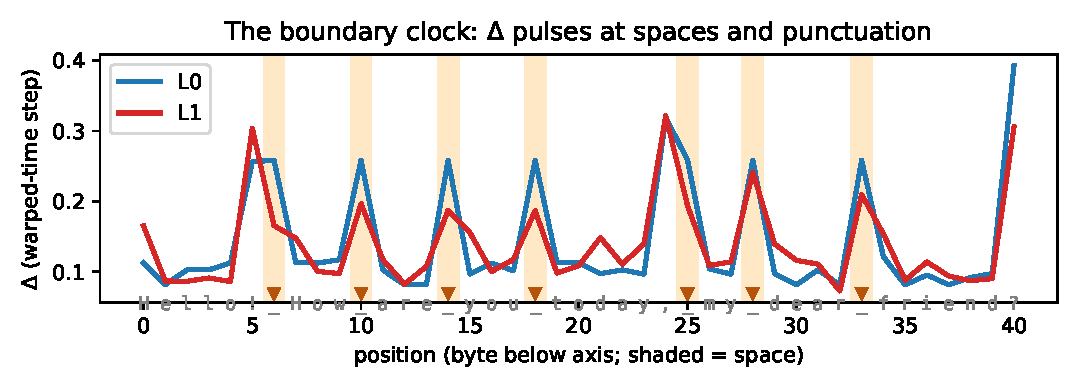
\includegraphics[width=\linewidth]{figures/fig_clock.pdf}
\caption{The boundary clock on a held-out sentence: $\Dt$ (mean over
channels, both layers) pulses at spaces and punctuation (hatched bands and
triangle markers = space positions). \emph{The clock is real and byte-keyed --- the
model ticks faster at word boundaries.}}
\label{fig:clock}
\end{figure}

\paragraph{Cross-architecture.}
Trained Mamba-2 develops boundary-responsive gating too --- with the
\emph{opposite operation}: its per-head $\Dt$ at spaces drops to
$0.13$--$0.65\times$ the letter mean, and its ZOH write magnitude to
$0.15$--$0.70\times$ in the deep layers (the input layer goes the other
way, $1.4\times$). Both models are
parameter-matched to \wskan{} (tier configurations in Appendix~E), byte-level, same data, same
training budget; the mamba2 granularities differ by design (per-head
pooled $\Dt$ vs per-channel). Mamba-2 \emph{skips}
boundaries; \wskan{} \emph{resets} at them. The comparison is causal on
both sides: forcing Mamba-2's $\Dt$ at spaces up to the letter mean damages
word-initial prediction $+0.28$ nats vs $+0.08$ at letter positions (a
matched control intervention shows the reverse asymmetry, $+0.19$ vs
$+0.29$) --- position-specific, though less sharply localized than
\wskan{}'s clock. And the
attention baseline inverts the asymmetry entirely: masking the transformer's
attention to boundary bytes costs word-initial CE $+2.93$, while masking
letters costs $+4.75$ ($0.62\times$) --- no special boundary dependence.
The comparison is not an artifact of
\wskan{} being underfit: at matched eval CE (Mamba-2 at 75k steps,
$1.182$ vs \wskan{}'s $1.184$), the same battery gives $+0.24$
word-initial damage for boundary removal against $+0.18$ for the matched
control --- the position asymmetry survives loss-matching, so the
sharpness gap between the two architectures' boundary mechanisms is
architectural, not a maturity artifact.
Boundary-responsive gating therefore appears in both SSM members we
tested --- with opposite operations and different $\Dt$ granularity
(per-head pooled vs per-channel). With two members and a structural
granularity confound, this is an existence observation, not a family-level
conclusion: the SSM family \emph{admits} boundary mechanisms, in at least
two opposed forms; whether language demands one is not answered here ---
a correction to our earlier framing, measured by the same battery on all
three. The causal protocol
is position-matched on both SSM architectures (raise $\Dt$ at the same
positions, measure the same quantity); what differs is the architecture's
own aggregation granularity (Mamba-2 pools 16 channels per head, \wskan{}
does not pool) --- that difference is part of what is being compared, and
we flag it as an interpretation of the sharpness gap, not a measurement.

\subsection{The oscillator bank}

The learned effective timescales $\rho_k \sigma_{ik}$ span a ladder
(geometric-fit $R^2$ 0.64--0.89 on the canonical tier's layers, from a
flat init; the full per-tier grid gives 0.60--0.97, Appendix~B; ratio
1.3--2.3$\times$)
whose slow tail reaches $\sim$3{,}190 tokens at the 10m tier while the
median half-life stays $\approx 1$ token at 100k. The tail carries $<1\%$
of readout weight --- present, unused.

\begin{figure}[t]
\centering
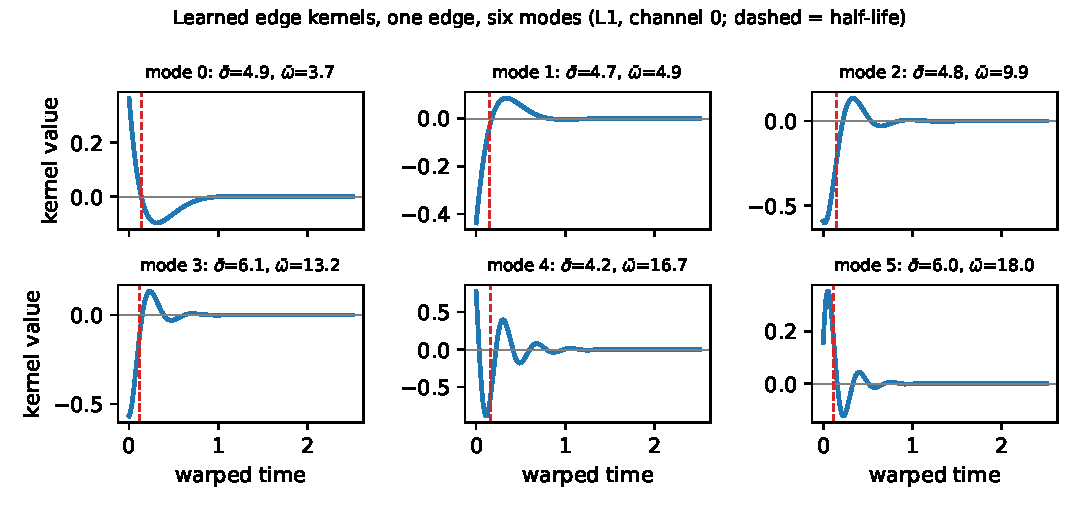
\includegraphics[width=\linewidth]{figures/fig_kernels.pdf}
\caption{One edge's six learned mode kernels (L1, channel 0, canonical
checkpoint) in warped time; dashed lines mark each mode's half-life.
Frequencies rise across modes; decays vary less. \emph{The
oscillator bank is a frequency ladder, learned.}
Population statistics
exist elsewhere ($|$DC$|$/RMS in \S\ref{sec:model}; ladder $R^2$ in
Appendix~B); this gallery shows what a single edge looks like.}
\label{fig:kernels}
\end{figure}

\subsection{Gates split structure from content}

The named rows of $M^B, M^C$ carry the discrete formatting bytes (digit,
newline, punctuation); the residual carries byte identity ($R^2$
$1.00 \to 0.76 \to 0.50$ with depth) and bigram statistics ($R^2$
0.91/0.84). At 10m the write path's non-bigram share is predominantly
\emph{trigram-level} statistics (cumulative explained variance $0.48
\to 0.65 \to 0.94$ over byte/bigram/trigram families; word identity adds
0.09; 5.4\% unidentified) --- scale growth is the \emph{order} of local
statistics, not a new object class.

\subsection{Decisions decompose exactly}
\label{sec:decision}

Additive residuals plus a linear tied head imply every decision margin
decomposes into named summands whose sum equals the margin \emph{exactly}
--- here and throughout, ``exact'' means no approximation in the
decomposition arithmetic: each summand is a computable part of the forward
pass, and the parts sum to the margin within floating-point tolerance
(asserted $< 10^{-4}$ on every use). \paragraph{Why the sum is exact (and what it does not claim).}
Let $x_{\text{fin}} = \mathrm{emb} + \sum_l (\mathrm{base}_l +
\mathrm{wave}_l)$ be the final residual stream. Every summand in the table
is a vector the forward pass itself computed --- the layer output
$\mathrm{out}_l$ is \emph{defined} as $\mathrm{base}_l + \mathrm{wave}_l$,
and the final LayerNorm is affine given the batch statistics:
$\mathrm{norm}(x) = \sum_v (v/\sigma)\cdot g + (\text{const})$ for any
additive decomposition $x = \sum_v v$. The table is therefore a
distribution of a sum the model actually performed --- it is exact for
every decision, not because any cancellation holds, and the integrity
assert ($<10^{-4}$) is checked on every decomposition we report (the
frien$\to$`d' case, the 50-per-tier truncation contexts, and all 150
benchmark contexts). What it does \emph{not} claim is causal
independence: $\mathrm{wave}_1$'s value already contains L0's influence
through the layer input, so a summand is the model's own computed part,
not a counterfactual contribution --- causal claims live in the
intervention battery (\S\ref{sec:clock}), which measures removals, not
summands.

Canonical case
\texttt{frien$\to$`d'} (margin $8.44$ over the runner-up `t'). The
decomposition's novelty is not the additivity --- any additive-residual
model has that --- but that here every summand is a \emph{named} object
(a mode's kernel, a gate's feature row), so the parts are readable, not
just computable:

\begin{center}
\begin{tabular}{lr}
\toprule
summand & margin contribution \\
\midrule
token embedding & $+0.83$ \\
L0 base (skip) & $+5.32$ \\
L0 wave (scan) & $-5.31$ \\
L1 base (skip) & $+0.88$ \\
\textbf{L1 wave (scan)} & $\mathbf{+7.50}$ \\
norm constant & $-0.79$ \\
\midrule
\textbf{sum} & $\mathbf{+8.44}$ \ (exact) \\
\bottomrule
\end{tabular}
\end{center}

\begin{figure}[t]
\centering
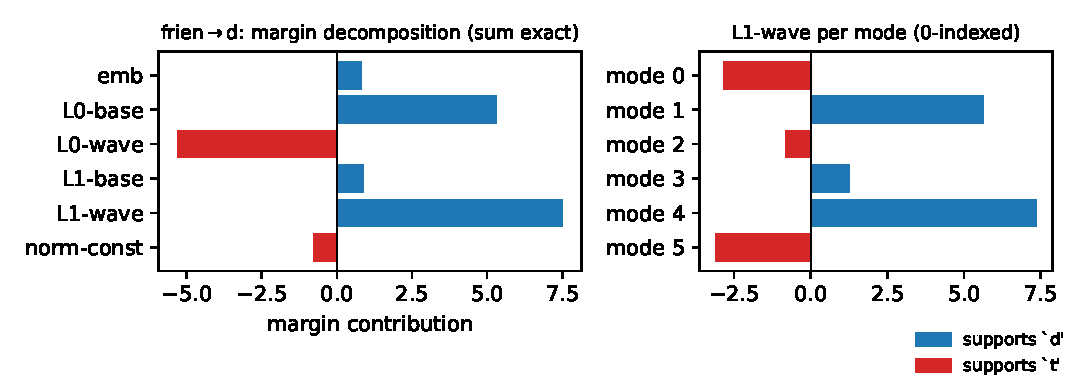
\includegraphics[width=\linewidth]{figures/fig_decision.pdf}
\caption{The same decision visually. Left: the exact margin decomposition
(parts sum to 8.44). Right: the L1-wave term per mode --- modes 4 and 1
(0-indexed) carry the completion here; mode identity is per-decision, not
a global semantics. \emph{Decisions are readouts of named parts,
not black-box logits.}}
\label{fig:decision}
\end{figure}

The decisive L1-wave term further decomposes per mode as
$[-2.85$, $+5.64$, $-0.81$, $+1.25$, $+7.36$, $-3.09]$.\footnote{Rounding
and precision notes. At two decimals the parts sum to $8.43$; the
three-decimal parts $+0.829$, $+5.321$, $-5.306$, $+0.879$, $+7.504$,
$-0.789$ sum to $8.438$ against a margin of $8.4392$, and the per-mode
list sums to $7.504$, matching the L1-wave part exactly. All measured in
fp32; the same forward pass in the bf16 training precision gives a margin
of $8.30$, a $0.14$ precision gap --- every analysis number in the paper
is fp32. The L0-base/L0-wave near-cancellation is a coincidence of this
decision: L0's residual output is $2.6\times$ its input norm here, far
from identity; the opposing votes are strong and happen to balance ---
they are not a conserved quantity.}
Mode identity is per-decision, not a global semantics: across 20
pre-registered completion contexts, the dominant path and modes vary
(\S\ref{sec:hand}).\footnote{A note on naming: ``modes 4 and 1 carry the
morphological completion'' (0-indexed) is a statement about \emph{this}
decision --- the context ends in \texttt{frien} and the answer completes
\texttt{friend}, so the positive modes are the ones driving the
completion here. The decomposition is exact arithmetic; the semantic
label attaches to the case, not to the mode --- the named modes here
illustrate the machinery at work on a real decision; they are not claimed
as a mode semantics.}
The recurring
pattern across decisions: word endings resolve as L1-over-L0 disagreement
resolutions (the shallow wave path resists, the deep one completes). The
same decision across tiers: 1k fails outright (predicts a space, margin
0.42), 10k succeeds by a hair (margin 0.08), then the margin strengthens
8.44 / 12.86 / 13.80 at 100k / 1m / 10m --- morphological completion is
the same mechanism, sharpened by scale.

\paragraph{The audit across tiers.}
The organization audit of \S\ref{sec:organization} is not 100k-only: the
surgical battery (all tiers) and the retrain test (10k, 1m, 10m, seed 42)
show the same verdict at every scale --- the named tables are surgically
load-bearing at small scale and nearly free at 10m ($+2.5 \to +0.05$
nats), the gauge symmetry is exact everywhere, and retraining without the
structure stays within $0.031$ nats of the baseline at every tier
tested. The detectability bounds are small in absolute terms
(0.04--0.10 nats, roughly 3--8\% of CE at these tiers) --- null results
are bounded, not exact zeros.

\subsection{Production}

In generation the same loop runs from the inside: the clock pulses at
boundaries, word-internal letters are wavelet-path decisions against a
negative token prior, and punctuation triggers a synchronized spike across
clock, paths, and modes.

\section{How the anatomy varies with scale (5 tiers $\times$ 5 seeds)}

\begin{figure}[t]
\centering
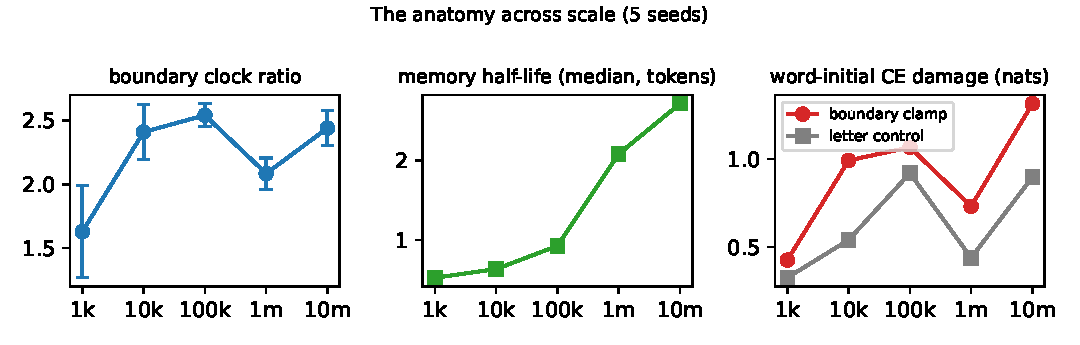
\includegraphics[width=\linewidth]{figures/fig_campaign.pdf}
\caption{The anatomy across scale (5 seeds): the clock ratio stays
$1.6$--$2.5$, memory grows with capacity, and the causal gap over the
matched control holds at every tier. \emph{The anatomy is not a
single-scale story.}}
\label{fig:campaign}
\end{figure}

The anatomy is consistent across the tiers measured (within this KAN
family, up to 10m --- nothing is claimed beyond it; the full 5-tier table
is Appendix~B). The surgical/retrain audit
(\S\ref{sec:organization}) runs at every tier for the surgery and at
10k/1m/10m for the retrains; only the circuit-level detail is 100k-only.

\begin{center}
\small
\begin{tabular}{lccc}
\toprule
tier & $\Dt$ ratio, space/letter (L1, 5 seeds) & half-life med (tok) & \texttt{frien$\to$`d'} \\
\midrule
1k & $1.63 \pm 0.40$ & 0.53 & 0/5 \\
100k & $1.95 \pm 0.27$ & 0.92 & 5/5 \\
10m & $2.48 \pm 0.14$ & 2.45 & 5/5 \\
\bottomrule
\end{tabular}
\end{center}

The causal word-initial effect exceeds its matched control at every tier:
$+1.12$--$4.02$ nats of damage against $+0.00$--$0.35$ for the control
($+2.50 \pm 1.00$ vs $+0.13 \pm 0.01$ nats at 100k). The differences, not
any ratio, are the headline: the near-zero control damage makes ratios
denominator-sensitive.
(The Mamba-2 comparison of \S\ref{sec:clock} --- position-specific on
both, sharply localized only in \wskan{} --- is not repeated here.)
The factor dips at 1m --- and the dip is causal, not metric: clamping the
boundary $\Dt$ to the letter mean at \emph{each single layer} damages
word-initial CE on \emph{every} layer of the 1m tier
($+0.13$--$0.39$ across L0--L5, s42, largest at the first and last
layer), while at 100k the same clamp is concentrated in the input
layer ($+3.19$ at L0 vs $+0.80$ at L1). The clock's causal role
redistributes with depth: distributed across all six layers at 1m,
concentrated at the input layer at 100k. The tier grid confounds depth
with capacity (the 1m tier is 6 layers, the 10m tier 2), so we ran the
control: a 6-layer model at 100k-tier capacity (109k params, 2 seeds)
shows the same clock at every layer ($\Dt$ ratios 1.4--3.2) with the
causal role partially spread but still input-layer-heavy (L0's share of
the total clamp damage 29--43\%, against 80\% for the 2-layer 100k and
19\% for the 6-layer 1m) --- depth spreads the role, capacity dilutes it
further, and the input layer remains the largest contributor at matched
capacity (\texttt{W12\_depth6\_analysis.py}). The second crossing of the
grid agrees: a 2-layer model at 1m-tier capacity (960k params, 2 seeds)
sits between the two, L0 share $\approx$60\% --- depth is the dominant
axis of the redistribution, capacity a secondary dilution
(\texttt{W12\_variant\_clocks.py}). The clock itself is present at
every layer of the tier
(per-layer space/letter $\Dt$ ratios 2.18 / 1.86 / 1.52 / 1.56 / 1.61 /
1.75).
The memory tail grows $4 \to 3{,}190$ tokens;
morphological competence appears only $\ge$ 100k. The wavelet's
performance contribution --- measured against \wskan{}-real, the identical
architecture with the oscillation frozen off ($\omega \equiv 0$); 73 of 75
paired cells --- is real, modest, and scale-shrinking: $-0.02\ldots -0.08$
nats at 1k--100k, $-0.01\ldots-0.03$ at 1m--10m.

\section{What the model does not represent linearly}
\label{sec:exclusion}

\noindent\fbox{\parbox{0.97\linewidth}{\textbf{Definition (operational, scale-conditional).}
\emph{Form} = the distributional regularities of the text surface ---
boundary timing, local n-gram statistics, morphological continuation.
\emph{Content} = reference: facts, entities, long-range meaning. The
boundary is our choice, marked rather than hidden; it is conditional on
the tiers measured (up to 10m, where content has loosened to trigram
order, no further).}}

\vspace{0.5em}
Morphological completion sits exactly on the boundary. We count
it as form because its measured machinery is local --- a boundary clock
and a per-decision mode vote over a handful of recent bytes --- with no
factual content; we do not claim morphology is \emph{only} surface
structure, and a reader who places it on the content side loses none of
the measurements, which are definition-independent. The boundary is also
falsifiable: if a future tier shows reference-level variables (facts,
entities, turn state) in the linearly accessible write path, the
``form-only'' claim dies; the 10m measurement (content loosens to trigram
order, no further) is where it currently stands. What the battery does
\emph{not} cover: facts, entities, coreference, and other long-range
semantics --- untested at every tier, and the honest reading of the 10m
trigram finding is that reference has not yet entered the local window,
not that it cannot at larger scale or on other tasks. The label names the
measured phenomenon compactly --- it does no work beyond that, and
deleting it changes no number below. Sensitivity: if
morphology is moved to the content side, the claims that move are the
label ``form-only'' and the morphological-completion examples; the clock,
the ladder, the gate split, the decomposition machinery, and the exclusion
results below all stand as measured.

Linear probes on the write path, measured at every tier (UltraChat, seed
42; script in Appendix~F):

\begin{center}
\small
\begin{tabular}{lccccc}
\toprule
predictor (linear $R^2$) & 1k & 10k & 100k & 1m & 10m \\
\midrule
byte identity & 0.80 & 0.83 & 0.44 & 0.35 & 0.48 \\
bigrams & 0.81 & 0.76 & 0.64 & 0.53 & 0.64 \\
word identity & 0.10 & 0.13 & 0.15 & 0.14 & 0.14 \\
\quad (in-sample shuffled-label null) & 0.08 & 0.08 & 0.08 & 0.08 & 0.08 \\
\quad (ridge, held-out, best $\alpha$) & $-0.00$ & 0.01 & 0.02 & 0.02 & 0.02 \\
sentence position (8-bin) & 0.05 & 0.03 & 0.01 & 0.01 & 0.02 \\
word identity, MLP held-out & 0.07 & 0.10 & 0.26 & 0.29 & 0.25 \\
\quad (shuffled-label control) & 0.04 & 0.03 & 0.02 & 0.01 & 0.01 \\
\bottomrule
\end{tabular}
\end{center}

Above the bigram level the pattern is scale-stable, and null calibration
sharpens rather than rescues it: word identity's in-sample $R^2$
(0.10--0.15) sits just above its shuffled-label null (0.08 at every tier
--- with 500 classes on 4k positions the in-sample null is high, a
calibration the table now reports), and a held-out ridge sweep puts the
linearly decodable share at $R^2 \lesssim 0.03$ at every tier, against
held-out $R^2$ up to 0.60 for byte identity and 0.20 for bigrams. The
small value is not probe overfitting: quadrupling the probe positions
(4k $\to$ 16k) leaves it in the same band (held-out $R^2$
$0.029$--$0.032$ at 100k and 10m, accuracy $3\times$ the shuffled null,
while the in-sample null falls $0.08 \to 0.04$ as expected).
Sentence position is absent ($\le 0.05$), and the nonlinear recovery
grows from toy levels (7\%) at 1k to $\approx$25--29\% at 100k--10m and
saturates.
At 100k we additionally probed the post-gate signal and the residual
stream: word-identity linear $R^2$ stays 0.15--0.16 (the gate does not
linearize), while the MLP recovers 23.4\%/21.5\% there. Nonlinear
exploitability by downstream gates remains open at every tier.
This linear-fails/nonlinear-succeeds
pattern is not specific to this model --- it is the expected relationship
between probe classes --- but here the readout structure is known, so the
pattern pins down a sharper statement that generic substrates cannot
support: \emph{word-level information is
present, but the model's own linear readout can use almost none of it}.
We scope the statement precisely, because the construction argument is
per-layer: the readout $C$ is linear in its own layer's state by
construction, but at depth $\ge 2$ the end-to-end state$\to$logit map is
\emph{not} linear (the SiLU gate and the LayerNorm see earlier layers'
outputs). The claim is therefore empirical, not architectural, and it
covers the whole path the head reads: the linearly decodable share of
word identity is small from the write path, the post-gate signal, and the
residual stream alike (in-sample $R^2 \approx 0.10$--$0.16$ against a
shuffled null of $0.08$; held-out ridge $R^2 \lesssim 0.03$ --- the gate does
not linearize). A direct alignment check makes the same point from the
readout side: the model's own sensitivity to the write path (the mean
loss-gradient direction over 2k positions, 100k tier) sits at
$|$cos$| = 0.14$ with the probe's principal word-identity direction ---
about $2\times$ the 240-dimensional null of $0.065$ --- so the readout
touches the word-identity direction weakly rather than not at all. (An
earlier draft's absolute wording --- ``never exposed'' --- is corrected
accordingly: the measured statement is ``weakly exposed, an order of
magnitude below the bigram level''.)
Decodable is not exploited: whether downstream
nonlinearities make use of it is open; the behavioral recall probe
(memorize-then-recall) fails identically on matched-size Mamba-2, so ``no
facts, no recall'' is a scale-level observation, not an architecture-level
one. A positive control now backs that reading: on an induction
(in-context copying) task the measurement does detect signal
(4--5\% accuracy against a 0.4\% chance level, $n{=}200$, on both
architectures) --- so the probe can see recall-type behavior when it
exists, and at this scale even local copying sits near the floor. The
recall null is a capability floor of the scale, fully consistent with the
370m IOI result \cite{ioi-mamba}, where the same model class does store
entities linearly. The stronger wording an earlier draft used (``provably'') is
retracted with the rest in \S\ref{sec:organization}.
(The word-initial decisions used in \S\ref{sec:benchmark} sit on the same
boundary: predicting a word's opening letter is distributional, not
referential, by the same operational criterion.)

Scope note on scale: the table above is already per-tier; at 10m the
linearly accessible content loosens one n-gram order (the write path's
non-bigram share is predominantly trigram-level; \S\ref{sec:anatomy}).
Trigrams stay \emph{form} by our criterion --- higher-order but still
local distributional statistics --- so the definition does not move at
10m; what moves is its order.

\section{Deriving the next token by hand}
\label{sec:hand}

An itemized from-scratch forward pass (serial scan, explicit warped-time
history sums, every gate value printed) reproduces the model's logits to
$3.8 \times 10^{-6}$ at the 1k/10k/100k tiers. At 1k (d$=$4, one layer)
the whole computation fits on a page: 576 history terms for a 24-byte
context. Worked example: after \texttt{``sunrise.\textbackslash n O''} the
model outputs `n' --- the decisive term is the period--newline pair closing the
previous sentence, read through mode 4 at warped distance 0.628 ($+5.37$ of the wave path's
$+9.26$). A near-miss (\texttt{"`Ow! Tha"'} $\to$ `n' for ``Than'' where
the text has ``That'') is equally legible.

The decision is a low-rank event at every scale: ranked by contribution,
the median context needs 12 / 26 / 6 / 1 / 2 history terms (of 576 /
1{,}728 / 11{,}520 / 17.7M / 37.7M) for the argmax to stabilize at
1k / 10k / 100k / 1m / 10m --- the median decision at 10m is settled by
\emph{two} of thirty-seven million history terms. Static parts alone
decide 10 / 14 / 26 / 50 / 30\% of contexts --- at 1k history is the
decision; at 1m half the decisions are already settled before history
sums. What this is
\emph{not}: derivation without execution. The gates are input-dependent
and must be computed; what exists is \emph{transparent simulation} ---
complete at 1k/10k, truncated at 100k+ (a median 6 of 11{,}520 top-ranked
terms then suffice to stabilize the argmax, Appendix~D).\footnote{Two
clarifications. First, practical scale: the complete 1k case is 576
scalar terms --- a full hand-check is hours of careful arithmetic, but
every step is printed and checkable; the median case needs 12. Second,
the clock is not contradicted by the tiny term counts: at the 10m tier
the dominating terms sit at their positional base rate (boundary bytes
hold 21\% of the top-25 terms vs a 20\% base rate); at smaller tiers
boundary positions are moderately \emph{over}-represented (28--47\% vs
20--24\%), consistent with the clock concentrating credit at resets
rather than contradicting it. Either way the clock sets the \emph{reach}
of every term through the warped-distance kernel.}

A pre-registered dictionary test at 100k (4-byte suffixes with $\ge 8$
observations and $\ge 75\%$ next-byte purity, 20 eval contexts): the model
matches the corpus completion 20/20 --- but the dominant path varies
(L1-wave only 8/20) and the canonical mode dictionary transfers to just
2/20. The object-level anatomy transfers; the per-decision semantic
inventory does not.

\subsection{Writing the model by hand}
\label{sec:handcraft}

The strongest test of an anatomy is constructive: can the edge functions
be \emph{written} by hand? We hand-set every parameter of a 1k-tier shell
from the measured anatomy alone --- the clock ratios, the ladder, the gate
split, a word-length integrator mode, a sentence memory --- with no
training (script \texttt{W12\_handcraft.py}; details in the handcraft
report). The result produces pseudo-text with real word boundaries, a
plausible length distribution, vowel/consonant texture, and case and
punctuation rhythm. The word-length mechanism is visible in a single
number series: the margin $\text{logit}(\texttt{space}) -
\text{logit}(\texttt{e})$ after $k$ consecutive letters runs $-11.44,
-8.26, -6.15, -3.81, -1.41, +2.91$ for $k = 1, 3, 4, 5, 6, 8$ ---
boundary pressure building as the word lengthens, the clock-plus-integrator
pattern of \S\ref{sec:clock} working in a model that has never seen data.

\begin{center}
\small
\begin{tabular}{lc}
\toprule
configuration & CE (TinyStories eval) \\
\midrule
hand-written, static skeleton only (emb + base + frequency-tilted head) & 7.53 \\
\textbf{hand-written, full} (static + form machinery) & \textbf{5.45} \\
unigram reference & 3.06 \\
trained 1k model & 2.23 \\
\bottomrule
\end{tabular}
\end{center}

The decomposition of the score is honest in both directions: the form
machinery is worth $-2.08$ nats over its own static skeleton, and the
skeleton itself is a bad prior (7.53 against the 3.06 unigram reference)
because a 4-dimensional output table cannot express a real unigram model
--- the remaining gap to unigram is output calibration, not mechanism,
and the gap to the trained 1k model (2.23) is the lexicon, which is what
training adds. The build's own failure modes were as informative as the
result: oscillatory slow modes destroy accumulation (hence zero $\omega$
on the integrators), sparse embeddings let the SiLU gate choke the wave
path (a dense-bias fix), and a LayerNorm mean-shift can counterfeit a
case channel --- each a named mechanism, found with the same decomposition
tools used on the trained model. Form by hand, content by data.

\section{Where the organization comes from}
\label{sec:organization}

The structures above exceed naive task requirements; we audited whether
they are required at all.

\paragraph{Solution-load $\neq$ task-requirement (the audit's core
result, one table).}
Destroying the structure in the trained solution is costly; retraining
without it is not. Eval-CE deltas:

\begin{center}
\small
\begin{tabular}{lccc}
\toprule
structure & surgery (this solution) & retrain (the task) & verdict \\
\midrule
named feature tables & $+5.5$ (to $+0.05$ at 10m) & $-0.002$ & not required \\
$\rho$ timescale ladder & $+0.13$--$0.33$ & $-0.001$ & not required \\
mode bank ($N{=}6 \to 1$) & --- & $+0.038$, $p=0.002$ & small, real \\
oscillation ($\omega$) & --- & $+0.037$, $p=3{\times}10^{-4}$ & small, real \\
$\pi$-harmonic prior & --- & $-0.002$ & unnecessary \\
\bottomrule
\end{tabular}
\end{center}

Surgery used 3 seeds $\times$ 3 permutations; retrains are paired per-seed
deltas (7 seeds for mode bank, 5 for oscillation, 3 for the nulls, which
sit inside their detectability bounds). A full mode permutation changes
nothing ($+10^{-8}$ nats, exact gauge at every tier): \emph{a mode is a
coherent object} --- the value is the within-mode consistency of
frequency, timescale, and gains, not the ordering. The scale story runs
the same way on both sides of the audit: surgically, the tables and the
ladder carry the solution at small scale and are nearly free at 10m
($+2.5 \to +0.05$ and $+0.35 \to +0.006$ nats); on retraining, no variant
exceeds $0.031$ nats at any tier (10k/1m/10m, seed 42). The
frequency--mode consistency is the exception that stays load-bearing
everywhere ($+1.6$--$+3.1$).

\paragraph{Learning curves: ``not required'' at every budget, not just at
convergence.}
A retrain null at full budget is compatible with the structure being an
inductive-speed advantage paid for in data. The retrain logs answer this
directly: evaluated on one shared eval surface (the ablation harness's
own, applied to the campaign's intermediate checkpoints), the nofeat and
flat-$\omega$ retrains track the baseline's eval CE at every measured
budget from 25k steps on --- step-matched gaps within $\pm 0.01$ nats
(flat-$\omega$ opens a small early gap, $+0.012 \pm 0.008$ at 25k steps,
closed by 50k), and the median data-overhead ratio is $0.84\times$ /
$1.08\times$ --- no measurable data penalty for removing the structure
(\texttt{W12\_learning\_curve.py}; the same-surface protocol matters: the
campaign and ablation logs use different eval sets, and mixing them
fabricates a spurious $+0.05$ gap). A mismatched-prior control completes
the separation: the named feature tables \emph{present but shuffled at
init} (the seven byte features permuted among themselves, trainable)
retrain to baseline as well --- paired per-seed deltas $+0.009, -0.006,
-0.012$ nats, mean $-0.003 \pm 0.010$ --- so it is not merely that the
structure can be absent; a \emph{wrong} assignment of the same structure
is equally free. And the basis itself is scaffolding: with the seven
named predicates replaced by a fixed, untrainable random partition of the
byte range (\texttt{scramfeat}, 2 seeds), the model retrains to baseline
($-0.005$ / $-0.011$ nats) and the \emph{same} boundary clock emerges
with the same causal profile ($\Dt$ ratios $2.2$--$2.7$, clamp damage
input-layer-concentrated) --- the clock does not read the gate basis, and
the gate basis carries no necessary linguistic value. The organization is
the solution's, not the task's.

\paragraph{Origin.}
\begin{figure}[t]
\centering
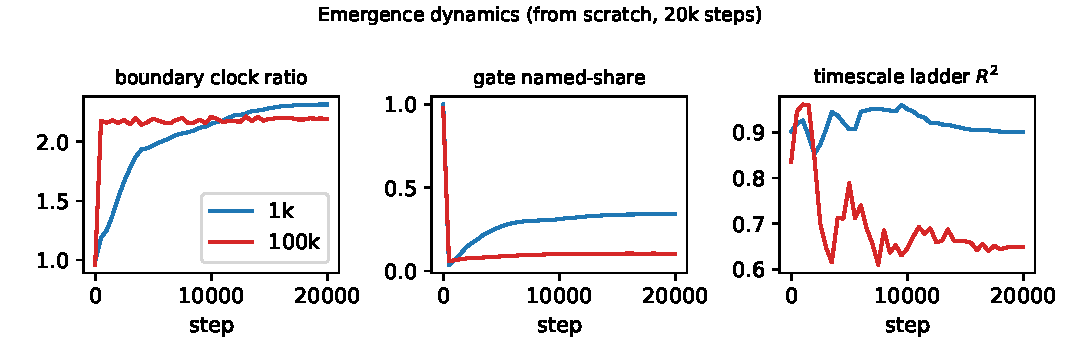
\includegraphics[width=\linewidth]{figures/fig_dynamics.pdf}
\caption{Emergence trajectories (from-scratch runs, 20k steps, 1k and 100k
tiers): the timescale organization is immediate, the clock follows within
hundreds to thousands of steps, the gate split re-equilibrates slowly.
\emph{The organization is built early, in a fixed order.}
Shown for illustration of the emergence order; these are
constant-learning-rate diagnostics, and the noisy 100k ladder-$R^2$ trace
carries no claim.}
\label{fig:dynamics}
\end{figure}
\textbf{Claim.} The frequency skeleton is an init prior ($\pi$-harmonics),
not destroyed by training --- and unnecessary.

\textbf{Evidence.} Flat-$\omega$ retrains (no harmonic prior, trainable)
match the baseline loss and rebuild a frequency ladder from zero
($R^2$ 0.83--0.96 by the geometric-fit statistic, now over the $\omega$
dimension --- a different object from the timescale ladder of
\S\ref{sec:anatomy}).
Everything else --- timescale ladder, boundary clock, gate split --- is
learned within a few hundred steps, without oscillation, and in analogous
form across architectures. Step-0 gradient anatomy (20 batches): the
embedding takes 94.7\% of the initial gradient, yet the per-mode gradient
of $\log\sigma$ is already non-uniform (CV $0.43 \pm 0.08$ / $0.28 \pm
0.05$) --- data breaks mode symmetry immediately, prior or not.

\textbf{Caveats.} The initial step scale ($\Dt_0 = 0.05$ by the softplus
bias init) is a \emph{necessary
condition} for the clock: with $\Dt_0 = 0.5$ it never emerges (10k steps).
The emergence ordering, from measured trajectories (the figure
illustrates; the claims rest on the numbers): timescale organization
within the first ~250 steps; content-residual growth next (gate
named-share collapses 1.0 $\to$ 0.02--0.14); the boundary clock emerges by
250 steps at 100k and 2--4k at 1k; the gate split re-equilibrates slowly
to a plateau (0.34 at 16--18k steps, 1k tier).

\paragraph{Retractions (lessons learned).}
Early drafts claimed the organization was task-required (retrain test:
no) and that channels form antipodal specialist pairs (position-shuffle
null: no). The causally load-bearing specialist singletons survive ---
e.g.\ the L0 boundary-detector channel, $+1.08$ CE when zeroed.
A masking bug in the first-pass implicit-boundary and per-layer clamp
batteries, caught in review, is also corrected here: it understated the
L0 necessity clamp ($+0.556$ reported; $+2.57 \pm 0.48$ corrected),
understated the 100k per-layer concentration ($+0.56/+0.13$ reported;
$+3.19/+0.80$ corrected), and perturbed the 1m per-layer spread and the
implicit-clamp comparison; all clamp numbers in the paper are the
corrected ones.

\paragraph{Why a language model at all.}
A synthetic task would show that hand-set gates \emph{can} organize; only
real text shows whether the organization gradient descent builds on
language statistics is the one we claim. The substrate has to touch the
data whose structure it is meant to reveal --- the clock, the ladder, and
the split are answers to byte text, not to a toy distribution.

\paragraph{Statement.}
The organization is the path of least resistance under this
parameterization --- immediately and reliably found (5-seed convergence of
coarse structure and of the sorted mode-value distribution, CV 3--15\%)
--- and barely required by the task (within this parameterization family).
That is precisely what makes it
analyzable: the model is a readable record of an equilibrium this
function family makes accessible --- offered by the parameterization, not
demanded by the data. A residual circularity deserves to be
named: the retrain test stays \emph{inside} this parameterization, so
``path of least resistance'' is established within the family --- the
cross-parameterization edge is left open: the Mamba-2 analogy
(\S\ref{sec:clock}) is an existence observation with a granularity
confound, not evidence about requirement.

\section{The benchmark substrate, demonstrated}
\label{sec:benchmark}

\noindent\fbox{\parbox{0.97\linewidth}{\textbf{Three quantities, kept separate.}
\emph{Arithmetic attribution} (what our decomposition gives): the exact
sum of the model's own computed parts --- no causality. \emph{Removal
sensitivity} (what LOO gives): the margin change when a byte is removed ---
exact for that question, by direct computation. \emph{Causal
contribution} (what interventions give): the effect of perturbing a
mechanism --- measured in \S\ref{sec:clock}, not in this section. The
benchmark scores methods against arithmetic attribution; it says nothing
about the other two.}}

\vspace{0.5em}
Five standard post-hoc attributions score against the arithmetic ground
truth on three decision categories (50 contexts each, plus the canonical
case of \S\ref{sec:decision}):

\begin{center}
\small
\begin{tabular}{lccc}
\toprule
method (Spearman $\rho$ vs exact) & morphology (50) & word-initial (50) & post-punct (50) \\
\midrule
gradient $\times$ input saliency & $0.80 \pm 0.09$ & $0.78 \pm 0.10$ & $0.65 \pm 0.11$ \\
integrated gradients & $0.77 \pm 0.10$ & $0.69 \pm 0.14$ & $0.51 \pm 0.12$ \\
attribution patching (EAP) & $0.30 \pm 0.28$ & $0.43 \pm 0.18$ & $0.16 \pm 0.21$ \\
replacement (random byte) & $0.54 \pm 0.19$ & $0.50 \pm 0.18$ & $0.36 \pm 0.18$ \\
leave-one-out (delete) & $0.42 \pm 0.18$ & $0.27 \pm 0.16$ & $0.30 \pm 0.16$ \\
\bottomrule
\end{tabular}
\end{center}

The ranking is stable across all three categories: gradient methods track
the arithmetic best, replacement-perturbation sits in the middle, deletion
worst --- and the whole grid degrades at post-punctuation decisions.
Attribution patching \cite{eap} --- the method family that targets causal
contribution, run here as single-position corruption with the standard
corrupted-run gradient --- lands between the gradient rows and the
perturbation rows ($\rho$ $0.16$--$0.43$). Under the three-way
distinction above this is the expected place for it: its answer is a
third quantity (an approximation of the counterfactual), and the table
quantifies how far that answer sits from the arithmetic readout it is
often identified with.
One confound we flag rather than resolve: gradient$\times$input and the
exact arithmetic share local-linear structure (both are first-order
objects of the same forward pass), so part of their agreement is expected
a priori. The cells that carry information beyond that shared structure
are the post-punctuation row, where every method degrades, and the
removal-based rows, which diverge everywhere.

A fair objection sharpened the finding: LOO answers ``removal
sensitivity'', and for that question it is \emph{exact} --- the margin
change under removal is directly computable, there is nothing for LOO to
be wrong about. The benchmark's content is therefore not ``LOO is
wrong'' but ``removal $\neq$ contribution'': the two questions diverge
measurably ($\rho \approx 0.3$), and a practitioner who reads removal
sensitivity as decision attribution is misled by exactly that much. The
gradient methods track the model's arithmetic far better than any
counterfactual method, and attribution patching --- the entry that
explicitly targets causal contribution --- lands between the two groups:
a third quantity, measured here rather than asserted. A linear probe concludes ``no word identity'' while the
substrate shows the information present but nearly linearly inaccessible
(\S\ref{sec:exclusion}). The section's claim is a measurement, not a new attribution
method: on a substrate where the answer is known, standard tools can be
graded.

\section{Related work}
\label{sec:related}

KANs \cite{kan} and their wavelet variants \cite{wavkan} motivate edges as
functions; SSMs and selective scan \cite{s4,mamba,ssd} motivate the
recurrent view --- \wskan{} identifies the two (an edge wavelet is an SSM
impulse response). Mechanistic interpretability \cite{clark2019} and
causal mediation \cite{rome} supply the post-hoc methods we benchmark
against; the documented unreliability of probes and attention-based
attribution \cite{hewitt-liang,jain-wallace} is what motivates having a
ground truth at all.
Within SSM interpretability specifically, the closest measurement is the
Mamba-2 state sink of \cite{mamba-sink}: boundary-token $\Dt$-gate
specialization at 2.7B scale, with the caution that perturbing the probed
$\Dt$ moves loss by at most $0.16$ nats while suppressing the same heads'
output moves it by $1.5$--$7.3$ --- an independent, much larger instance
of the removal/probe dissociation our benchmark measures
(\S\ref{sec:benchmark}). Their boundary class (BOS/newline, head-pooled
$\Dt$) differs from ours (spaces, per-channel $\Dt$): they find $\Dt$
\emph{elevated} at their boundary tokens where we measure it
\emph{suppressed} at spaces in Mamba-2's deep layers
(\S\ref{sec:clock}); the two are compatible --- different boundary
classes, granularity, and scale --- and the contrast is part of the
SSM-family variation that section reports. Circuit discovery transfers to
Mamba: \cite{ioi-mamba} partially reverse-engineers an IOI circuit and
finds entity names stored \emph{linearly} in the SSM state at 370m scale
--- against our linear-inaccessibility finding at byte scale
(\S\ref{sec:exclusion}); the difference (entity names in a templated task
at 370m vs word identity in running text at $\le$10m) is itself a
scale-and-task statement consistent with both. The hidden-attention view
of selective scan \cite{hidden-mamba} and the recall scaling laws of
\cite{mamba-recall} bound what SSM state can store, adjacent to our
scale-level no-recall observation. Gradient-based attribution patching
\cite{eap} is the method family \S\ref{sec:benchmark} grades against exact
answers.
Closest in spirit is the edge-function audit of a
B-spline KAN language model \cite{kan-lm-audit}, which reconstructs,
ranks, and prunes all feed-forward edge functions of a small LM and finds
them mostly active and smoothly low-dimensional (their top-4 functional
PCA components explain 99.9\% of edge-curve variance at their grid-2
setting --- a property their grid sweep shows is basis-imposed, not
learned: a fresh grid-2 init already gives 99.9\%, their \S4.1 control
analysis). Their own caveat --- that causal circuit claims would require
separate interventions --- is the gap our intervention battery fills. Our edges are a different object: temporal SSM impulse responses
with recurrence, whose readout-gain matrices are full-rank (effective rank
$\approx$ 35--37 of 40 per mode in the canonical layer) --- not
low-dimensional in their sense. (Full-rank gains do not make the model
less readable here: the readable unit is the named mode --- its timescale
and frequency --- and the per-mode attribution of \S\ref{sec:decision},
not the gain matrix's compressibility.) The two works are complementary views of
the KAN interpretability premise: static edge audit vs recurrent mechanism
anatomy. Basin selection connects to the lottery-ticket literature
\cite{lth}, and the post-hoc reliability debate to
\cite{wiegreffe-pinter,geirhos}. Within this intersection --- a trained
byte-level LM with SSM-parameterized recurrent edge functions --- we know
of no prior artifact whose edge functions are individually read, causally
tested, and decomposed to the logit margin; broader novelty claims we do
not make.

\section{Limitations}

\textbf{Scale and task.} Byte-level, up to $\approx$10m parameters, three datasets;
the anatomy is consistent across measured tiers within this KAN family,
and nothing is claimed beyond them. The computation is form-only ---
reference-level content was not found at any tier measured, and larger
scales could move it into the local window; the boundary is our
operational, scale-conditional choice.
\textbf{Seeds and power.} 3--7 seeds per retrain family (the headline
causal battery is $n{=}5$ seeds); nulls are bounded by detectability
(0.04--0.10 nats, 3--8\% of CE), not exact zeros; the benchmark demo
covers 3 categories $\times$ 50 contexts and 5 methods.
\textbf{Coverage.} Circuit-level analyses and the surgical/retrain audit
are 100k-centric (the per-tier batteries cover clock, memory, margins,
truncation --- not the full circuit detail).
\textbf{Family.} ``Barely task-required'' is established within this
parameterization family; the cross-family edge rests on the Mamba-2 and
transformer comparisons. The trade-off is one line: at the 100k and 10m
tiers the architecture costs 0.02--0.12 nats of CE against matched
baselines (more at the smallest tiers), and what it buys is
end-to-end auditability --- that is the whole exchange, stated without
inflation.
\textbf{Statistics strategy.} Effect sizes with seed-std for campaign
tables; paired per-seed deltas with t-tests for retrains, Holm--Bonferroni
over the 5-variant family (corrected $p = 0.0015$, $0.008$); sign tests
where direction is the claim; explicit null distributions where a
structure claim could be a metric artifact (the antipodal retraction used
a position-shuffle null). For the null retrains we report detectability
instead of zero: at 80\% power the nofeat / $\rho$-ladder / flat-$\omega$
tests would have resolved effects of $\ge 0.04$ / $0.09$ / $0.05$
nats --- ``not measurable at this noise level'' means smaller than that,
not exactly zero. No conclusion depends on a lone borderline test.

\section{Conclusion}

A language model whose edges are wavelets can be read like an instrument
panel, and --- at small scale --- its next token can be derived by
transparent simulation (complete below 10k parameters, truncated above),
or rebuilt by hand from the anatomy alone (\S\ref{sec:handcraft}). The
instrument panel is real, and it is not a dictionary: the object-level
anatomy transfers across decisions; the per-decision semantic inventory
does not (20/20 behavioral fidelity, 2/20 dictionary transfer). The organization that makes this possible is
neither required nor performance-optimal, and it is not the data's
fingerprint: present or mislabeled, the task retrains without it. It is
what the parameterization offers. We offer the artifact, the exact
methods, a grading of five standard post-hoc attribution methods against
exact arithmetic on it, and,
as lessons learned, several of
our own claims corrected or retracted along the way (listed in
\S\ref{sec:organization}).

\begin{thebibliography}{99}
\bibitem{kan} Liu, Z., Wang, Y., Vaidya, S., et al. KAN: Kolmogorov-Arnold
Networks. arXiv:2404.19756, 2024.
\bibitem{wavkan} Bozorgasl, Z., Chen, H. Wav-KAN: Wavelet
Kolmogorov-Arnold Networks. arXiv:2405.12832, 2024.
\bibitem{s4} Gu, A., Goel, K., R\'e, C. Efficiently Modeling Long
Sequences with Structured State Spaces. arXiv:2111.00396, 2021.
\bibitem{mamba} Gu, A., Dao, T. Mamba: Linear-Time Sequence Modeling with
Selective State Spaces. arXiv:2312.00752, 2023.
\bibitem{ssd} Dao, T., Gu, A. Transformers are SSMs: Generalized Models
and Efficient Algorithms Through Structured State Space Duality.
arXiv:2405.21060, 2024.
\bibitem{clark2019} Clark, K., Khandelwal, U., Levy, O., Manning, C. D.
What Does BERT Look at? An Analysis of BERT's Attention.
arXiv:1906.04341, 2019.
\bibitem{rome} Meng, K., Bau, D., Andonian, A., Belinkov, Y. Locating and
Editing Factual Associations in GPT. arXiv:2202.05262, 2022.
\bibitem{lth} Frankle, J., Carbin, M. The Lottery Ticket Hypothesis:
Finding Sparse, Trainable Neural Networks. arXiv:1803.03635, 2018.
\bibitem{hewitt-liang} Hewitt, J., Liang, P. Designing and Interpreting
Probes with Control Tasks. arXiv:1909.03368, 2019.
\bibitem{jain-wallace} Jain, S., Wallace, B. C. Attention is not
Explanation. arXiv:1902.10186, 2019.
\bibitem{kan-lm-audit} Alves, F., Vicente, R. Kolmogorov--Arnold Networks
for Small Language Models. arXiv:2607.15525, 2026.
\bibitem{wiegreffe-pinter} Wiegreffe, S., Pinter, Y. Attention is not not
Explanation. arXiv:1908.04626, 2019.
\bibitem{geirhos} Geirhos, R., Jacobsen, J.-H., Michaelis, C., et al.
Shortcut Learning in Deep Neural Networks. arXiv:2004.07780, 2020.
\bibitem{mamba-sink} Jiang, Y., Zhang, B. A Circuit, Not The Circuit:
Non-Unique Causal Localisation of the Mamba-2 State Sink.
arXiv:2606.00930, 2026.
\bibitem{ioi-mamba} Ensign, D., Garriga-Alonso, A., et al. Investigating
the Indirect Object Identification Circuit in Mamba. arXiv:2407.14008,
2024.
\bibitem{hidden-mamba} Ali, A., Zimerman, I., Wolf, L. The Hidden
Attention of Mamba Models. arXiv:2403.01590, 2024.
\bibitem{mamba-recall} Koren, Y., Ben-Kish, A., Giryes, R., Wolf, L.,
Zimerman, I. On the Recall Scaling Laws in Mamba: A Theoretical and
Mechanistic Study via Hashing. arXiv:2609.07681, 2026.
\bibitem{eap} Syed, A., Rager, C., Conmy, A. Attribution Patching
Outperforms Automated Circuit Discovery. arXiv:2310.10348, 2023.
\end{thebibliography}

\appendix

\section{Units and the representative-mode tuple}

All dynamical quantities live in warped-time units ($\sum \Dt$). Marginal
medians on the canonical checkpoint: L0 $\tilde\sigma \approx 5.7$,
$\tilde\omega \approx 9.9$; L1 $\tilde\sigma \approx 5.6$,
$\tilde\omega \approx 11.4$; $\bar\Dt \approx 0.11$--$0.15$. Per-mode
identities are exact by construction; medians of the correlated quantities
do not satisfy them (median of a ratio $\neq$ ratio of medians). All
ratios quoted elsewhere in the paper are ratios of \emph{means}
($\Dt$ at spaces vs letters), which are well-defined point estimates.
Representative exact tuple (L1, channel 0, mode 3 --- an arbitrary choice;
the identity holds for every mode by construction): $\tilde\sigma = 6.107$,
$\tilde\omega = 13.169$, $\bar\Dt = 0.153$ $\Rightarrow$ $Q = 1.078$,
$t_{1/2} = 0.740$ tokens, $0.321$ cycles/token.

\section{The anatomy at every scale}

\begin{center}
\small
\begin{tabular}{lccccl}
\toprule
tier & $\Dt$ ratio, space/letter (L1) & half-life med & half-life max & word-initial vs control & \texttt{frien$\to$`d'} \\
\midrule
1k & $1.63 \pm 0.40$ & 0.53 & 4 & $+1.70$ vs $+0.00$ & 0/5 \\
10k & $2.41 \pm 0.24$ & 0.63 & 2$^*$ & $+4.01$ vs $+0.01$ & 2/5 \\
100k & $1.95 \pm 0.27$ & 0.92 & 69 & $+2.50$ vs $+0.13$ & 5/5 \\
1m & $1.71 \pm 0.05$ & 1.28 & 92 & $+1.12$ vs $+0.20$ & 5/5 \\
10m & $2.48 \pm 0.14$ & 2.45 & 3190 & $+3.16$ vs $+0.35$ & 5/5 \\
\bottomrule
\end{tabular}
\end{center}
($^*$the 10k half-life max $=2$ is a single-layer-tier artifact --- no
second layer to host slow modes; the 10k median stays on the monotone
trend regardless. 5 seeds each; UltraChat.)

The rest of the anatomy, per tier (seed 42): the clock lives on every
layer at every tier (at the 6-layer 1m tier the per-layer ratios are
[2.18, 1.86, 1.52, 1.56, 1.61, 1.75]); the timescale ladder is geometric
at every layer (fit $R^2$ 0.60--0.97); the byte manifold separates classes
everywhere (within/between cosine gap 0.09--0.17); the gate named-share
declines with capacity (0.40/0.26 at 1k/10k $\to$ 0.07/0.007 at 10m ---
bigger models lean less on the named tables, consistent with the retrain
finding that they are not required). \emph{The objects are present at
every tier we measured; their dimensions and reliance patterns are not.}

\section{Performance context (byte-level cross-entropy, 5 seeds)}

Context, not a claim of superiority: Mamba-2 leads 12 of the 15 cells
(the four smallest tiers on all three datasets, plus 10m TinyStories and
10m UltraChat), the transformer leads 1m TinyStories and 10m WikiText, and
\wskan{} leads 1m UltraChat clearly and 1m WikiText by $0.0002$ nats ---
a tie within seed noise. (An earlier draft of this table claimed the full
1m tier; the campaign numbers do not support that, and the rows are now
included below.)

\begin{center}
\begin{tabular}{lcccc}
\toprule
tier (dataset) & \wskan{} & \wskan{}-real & Mamba-2 & transformer \\
\midrule
100k (TinyStories) & $0.776{\pm}.008$ & $0.812{\pm}.005$ & $\mathbf{0.747{\pm}.004}$ & $0.836{\pm}.020$ \\
100k (UltraChat) & $1.184{\pm}.021$ & $1.230{\pm}.018$ & $\mathbf{1.158{\pm}.019}$ & $1.288{\pm}.027$ \\
100k (WikiText) & $1.303{\pm}.012$ & $1.344{\pm}.008$ & $\mathbf{1.282{\pm}.010}$ & $1.397{\pm}.021$ \\
1m (TinyStories) & $0.581{\pm}.010$ & $0.592{\pm}.007$ & $0.639{\pm}.008$ & $\mathbf{0.559{\pm}.012}$ \\
1m (UltraChat) & $\mathbf{0.934{\pm}.010}$ & $0.957{\pm}.011$ & $1.010{\pm}.022$ & $0.973{\pm}.056$ \\
1m (WikiText) & $\mathbf{1.110{\pm}.007}$ & $1.128{\pm}.009$ & $1.170{\pm}.012$ & $1.110{\pm}.029$ \\
10m (TinyStories) & $0.546{\pm}.005$ & $0.558{\pm}.004$ & $\mathbf{0.478{\pm}.007}$ & $0.487{\pm}.009$ \\
10m (UltraChat) & $0.833{\pm}.006$ & $0.861{\pm}.007$ & $\mathbf{0.716{\pm}.007}$ & $0.799{\pm}.027$ \\
10m (WikiText) & $1.023{\pm}.017$ & $1.045{\pm}.019$ & $0.948{\pm}.020$ & $\mathbf{0.940{\pm}.015}$ \\
\bottomrule
\end{tabular}
\end{center}

\section{Hand-simulation truncation curve}

50 held-out 24-byte contexts per tier; terms ranked by contribution to the
predicted byte's logit; ``static alone'' = embedding + base + norm parts
only.

\begin{center}
\begin{tabular}{llccccc}
\toprule
tier & ($d$, $L$) & history terms & static alone & median terms & $\le 25$ terms & p90 \\
\midrule
1k & (4, 1) & 576 & 10\% & 12 & 76\% & 38 \\
10k & (12, 1) & 1{,}728 & 14\% & 26 & 50\% & 135 \\
100k & (40, 2) & 11{,}520 & 26\% & 6 & 74\% & 97 \\
1m & (80, 6) & 17.7M & 50\% & 1 & 80\% & 44 \\
10m & (512, 2) & 37.7M & 30\% & 2 & 78\% & 61 \\
\bottomrule
\end{tabular}
\end{center}

The count is non-monotone in size (12, 26, 6) because it tracks decision
\emph{sharpness}, not term count: the mean top-1--top-2 margin on these
contexts grows $0.94 \to 1.15 \to 2.37$ across the three tiers, and a
larger margin means fewer terms suffice to fix the argmax. The 10k tier
--- still single-layer but wider --- sits in the least sharp regime
relative to its term budget. Note the direction this implies for
hand-verifiability: the complete term-by-term verification lives in the
\emph{least} sharp regime (1k, where a median 12 terms still suffice);
sharpness is what makes the big tiers' decisions cheap to follow but also
is what training adds.

\section{Training protocol}

All runs are byte-level, tied embeddings, AdamW, grad-clip 1.0, cosine
schedule. Datasets: TinyStories, UltraChat-200k (byte stream), WikiText-103.
Campaign: $\approx$3-epoch budgets at the 100k tier (2.6--3.0 epochs);
capacity-tiered step caps at the other tiers (0.3--2.0 epochs), matched
across models per (tier, dataset); seeds 42/7/123/2024/31337.
Model tiers (wskan11: $d$, layers): 1k (4, 1), 10k (12, 1), 100k (40, 2),
1m (80, 6), 10m (512, 2); matched-size Mamba-2 / transformer / conv / lstm
baselines. Batch 64, block 256 (TinyStories/WikiText) or 512 (UltraChat);
lr $3{\times}10^{-3}$ ($\le$100k) or $10^{-3}$ (1m+); bf16 scan in
training, fp32 in analysis. The canonical analysis checkpoint is
\texttt{wskan11\_ultrachat\_100k\_3ep\_} \texttt{s42}. Analysis scripts
and measured numbers: \texttt{experiments/} and
\texttt{experiments/figures/}.

\section{Reproduction map}

\begin{sloppypar}
Code and checkpoints: \url{https://github.com/llaa33219/wskan}. The 15
campaign checkpoints of the released family (5 sizes $\times$ 3 datasets,
seed 42) are also published as safetensors on Hugging Face,
\texttt{llaa33219/wskan-\{size\}-\{dataset\}} with \texttt{size} $\in$
\{1k, 10k, 100k, 1m, 10m\} and \texttt{dataset} $\in$ \{tinystories,
ultrachat, wikitext\} (e.g.\
\url{https://huggingface.co/llaa33219/wskan-10m-ultrachat}); each model
card carries its \texttt{config.yaml}, real generation outputs, and a
runnable one-command inference path
(\texttt{experiments/RELEASE\_infer.py}), and the published weights are
verified to regenerate those outputs byte-exactly
(\texttt{experiments/RELEASE\_verify.py}). Every
quantitative claim maps to a script in \texttt{experiments/} (script names
carry the project's version-era prefixes, V1\ldots W12; each maps to the
analysis it runs, below). Figures are generated from the checkpoints by
\texttt{experiments/W11\_paper\_figures.py} and must be present in
\texttt{paper/figures/} for compilation. Checkpoints
live under \texttt{checkpoints/} (campaign tier
\texttt{wskan11\_*\_3ep\_s*}); measured numbers under
\texttt{experiments/figures/}. The table below maps claim to script.
\end{sloppypar}

\begin{center}
\small
\begin{tabular}{ll}
\toprule
claim & script \\
\midrule
clock field, gate splits, units (\S\ref{sec:anatomy}) & \texttt{W7BC\_canonical\_probe.py} \\
causal battery, 5 seeds (\S\ref{sec:clock}) & \texttt{W11\_all\_sizes\_analysis.py} \\
clock sufficiency (false ticks; V6-era, 3 seeds) & \texttt{V6\_causal\_clock\_full.py} \\
production trace & \texttt{W7BC\_generation\_analysis.py} \\
ablation + performance tables & \texttt{CAMPAIGN\_aggregate.py} \\
all-sizes anatomy (Appendix~B) & \texttt{W11\_all\_sizes\_analysis.py} \\
hand-simulation (\S\ref{sec:hand}, Appendix~D) & \texttt{W11\_hand\_simulation.py} \\
exclusion battery + probes (\S\ref{sec:exclusion}) & \texttt{W11\_round5\_probes.py} \\
interventions, init-vs-trained, dynamics (\S\ref{sec:organization}) & \texttt{W11\_excess\_structure.py} \\
per-tier surgery; per-layer causal clamp & \texttt{W11\_surgery\_all\_tiers.py} \\
retrain test (\S\ref{sec:organization}) & \texttt{W11\_ablation\_retrain.py} \\
seed convergence; antipodal permutation null & \texttt{W11\_round7\_probes.py} \\
basin origin & \texttt{W11\_basin\_origin.py} \\
benchmark demo (\S\ref{sec:benchmark}) & \texttt{W11\_benchmark\_demo.py} \\
attribution-patching benchmark row (\S\ref{sec:benchmark}) & \texttt{W12\_benchmark\_ap.py} \\
Mamba-2 causal battery (\S\ref{sec:clock}) & \texttt{W11\_mamba2\_causal.py} \\
transformer boundary causal test (\S\ref{sec:clock}) & \texttt{W11\_tf\_causal.py} \\
5-seed clamp; implicit-boundary clock test & \texttt{W11\_implicit\_boundary.py} \\
5-seed implicit-boundary extension (\S\ref{sec:clock}) & \texttt{W12\_implicit\_boundary\_5seed.py} \\
null-calibrated probes; readout alignment (\S\ref{sec:exclusion}) & \texttt{W12\_probe\_nulls.py} \\
learning-curve retrain analysis (\S\ref{sec:organization}) & \texttt{W12\_learning\_curve.py} \\
mismatched-prior retrain control (\S\ref{sec:organization}) & \texttt{W11\_ablation\_retrain.py} \texttt{--variant shuffeat} \\
depth-confound control (\S\ref{sec:anatomy} scale section) & \texttt{W11\_ablation\_retrain.py} \texttt{--variant depth6}; \texttt{W12\_depth6\_analysis.py} \\
loss-matched Mamba-2 battery (\S\ref{sec:clock}) & \texttt{W12\_mamba2\_causal\_lossmatched.py} \\
architecture-level basis scramble (\S\ref{sec:organization}) & \texttt{W11\_ablation\_retrain.py} \texttt{--variant scramfeat}; \texttt{W12\_variant\_clocks.py} \\
2-layer skeleton at 1m capacity (\S\ref{sec:anatomy}) & \texttt{W11\_ablation\_retrain.py} \texttt{--variant wide2}; \texttt{W12\_variant\_clocks.py} \\
recall-probe positive control (\S\ref{sec:exclusion}) & \texttt{W12\_recall\_positive\_control.py} \\
probe robustness at 16k positions (\S\ref{sec:exclusion}) & \texttt{W12\_probe\_word16k.py} \\
\bottomrule
\end{tabular}
\end{center}

\end{document}

